

\begin{center}
    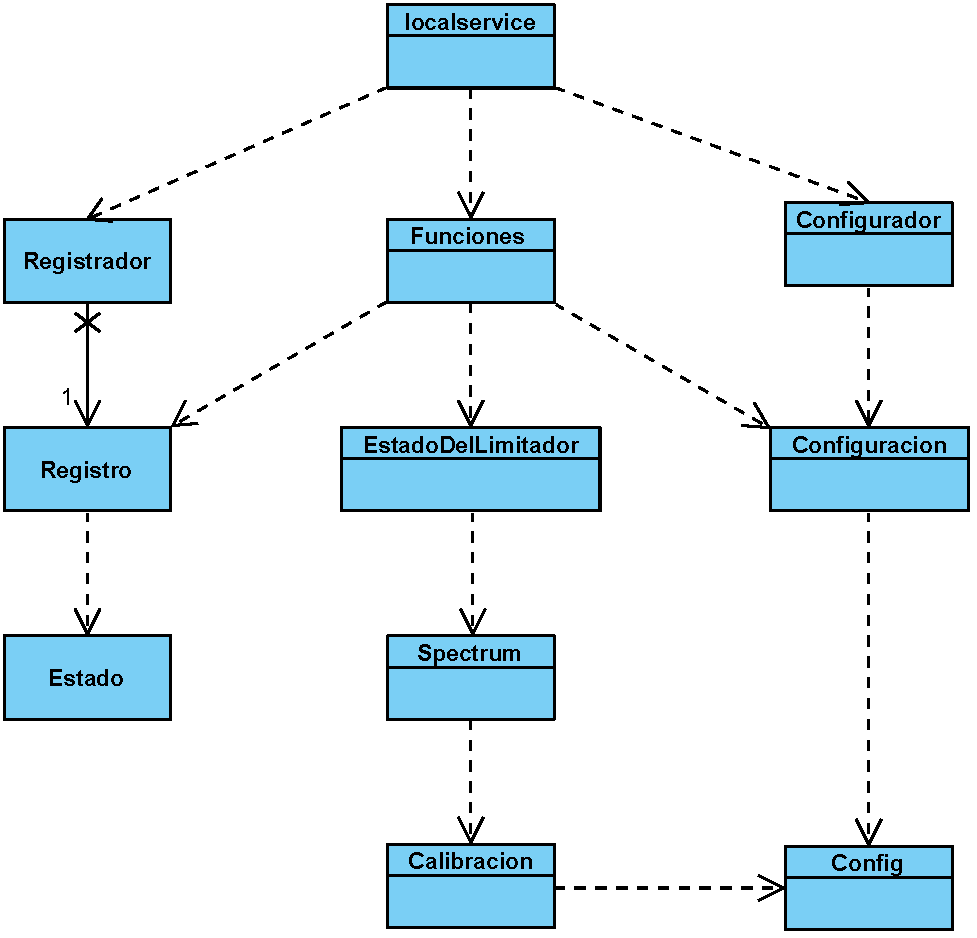
\includegraphics[width=0.9\textwidth]{figuras/lms9-localservice.pdf}
    \captionof{figure}{Diagrama de dependencias del programa localservice.}
    \label{fig:localservice}
\end{center}

Al igual que \verb|utilslr| recibe una serie de comandos como parámetro para modificar y consultar los datos del limitador. Los datos se devuelven \textbf{sin formato} útil (no JSON). El programa resulta excesivamente complejo, ya que contiene más del 1000 líneas de código, y ofrece funcionalidades que ya realizan otros de los programas auxiliares. Este programa pretende funcionar como un intérprete de comandos o una consola remota. Puede abrir y mantener un socket HTTP si se compila con las banderas requeridas.

Aunque el programa se llama \verb|localservice|, la clase principal se llama \verb|ServidorSerie|.

A continuación se listan los comandos que puede recibir este programa. Aquellos resaltados en negrita representan funcionalidad útil que ha sido exportada al LM11. Es fácil observar que mucha de las funcionalidades que ofrece este programa también la ofrecen otros programas auxiliares mucho menos complejos que este, y no solo eso, sino que mismamente dentro programa hay funcionalidad duplicada.

Comandos vía argumentos:
\begin{itemize}
	\item \textbf{calibralineas}: calibra el micrófono y las líneas.
	\item \textbf{miceq}: devuelve la ecualización del micrófono.
	\item \textbf{lefteq}: devuelve la ecualización de la línea izquierda.
	\item \textbf{righteq}: devuelve la ecualización de la línea derecha.
	\item \textbf{mic} \$float: re-calibra el micrófono con el valor recibido.
	\item \textbf{lefteq} \$float[8]: actualiza la ecualización de la línea izquierda con los valores recibidos.
		\subitem Los valores se dan separados por comas.
	\item \textbf{righteq} \$float[8]: actualiza la ecualización de la línea derecha con los valores recibidos.
		\subitem Los valores se dan separados por comas.
\end{itemize}

Comandos vía intérprete:
\begin{itemize}
	\item datos: permite modificar los datos del local.
	\item update: descarga y aplica la actualización dada una URL.
	\item configuración: muestra la configuración.
	\item configura: permite modificar parte de la configuración.
	\item actva: activa o desactiva el sistema.
	\item concha: abre conexión a telnet en el puerto 1036. Promociona la conexión.
	\item concharemota: abre conexión al terminal remoto en sheel.boanergesnetwork.com con la utilidad \verb|nc|.
	\item identifica: login.
	\item \textbf{calibra}: calibra un sensor manualmente.
	\item prepara:
		\begin{itemize}
			\item Muestra la configuración.
			\item Permite borrar la configuración.
			\item Permite cambiar datos del local.
			\item Permite inicializar el registro.
			\item Permite cambiar parte de la configuración.
		\end{itemize}
	\item operativo:
		\begin{itemize}
			\item Muestra la configuración.
			\item Permite cambiar algunos datos de la configuración.
		\end{itemize}
	\item \textbf{test}: calibra las líneas.
\end{itemize}